% Survey Overview / Structure Map — Standalone TikZ
% Compile: pdflatex survey_overview_tikz.tex
% Output: survey_overview_tikz.pdf -> rename to survey_overview.pdf

\documentclass[tikz,border=5pt]{standalone}
\usepackage{tikz}
\usetikzlibrary{shapes.geometric,arrows.meta,positioning,shadows,fit,backgrounds}

\definecolor{cblue}{HTML}{003f87}
\definecolor{cred}{HTML}{c0392b}
\definecolor{cgreen}{HTML}{1a7a4a}
\definecolor{corange}{HTML}{e67e22}
\definecolor{cgray}{HTML}{7f8c8d}
\definecolor{lcyan}{HTML}{d6eaf8}
\definecolor{lgreen}{HTML}{d5f5e3}
\definecolor{lorange}{HTML}{fdebd0}
\definecolor{lgray}{HTML}{f2f3f4}

\tikzset{
  secbox/.style={
    rectangle, rounded corners=4pt, draw=#1, fill=#1!10,
    text width=2.4cm, align=center, font=\scriptsize\bfseries,
    minimum height=0.85cm, drop shadow, inner sep=4pt
  },
  arrow/.style={-{Latex[length=2.5mm]}, thick, color=cgray},
  dottedflow/.style={-{Latex[length=2mm]}, dashed, color=cgray!60, thick}
}

\begin{document}
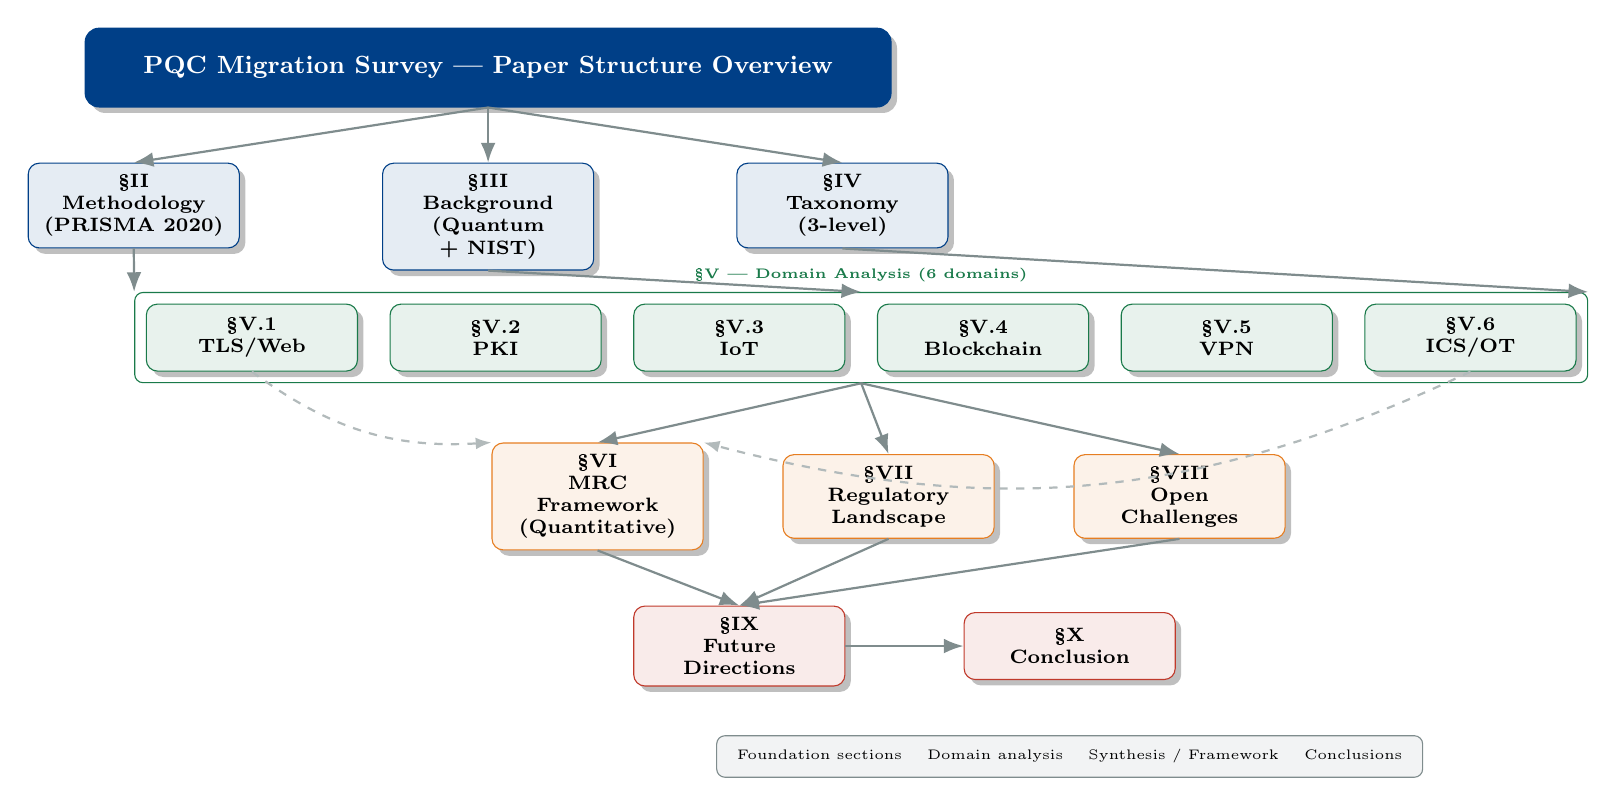
\begin{tikzpicture}[node distance=0.55cm and 0.6cm]

%── ROW 0: Title box ─────────────────────────────────────────────────────────
\node[rectangle, rounded corners=5pt, draw=cblue, fill=cblue, text=white,
      text width=10cm, align=center, font=\small\bfseries,
      minimum height=1.0cm, drop shadow] (title) at (0,0)
  {PQC Migration Survey — Paper Structure Overview};

%── ROW 1: Methodology ────────────────────────────────────────────────────────
\node[secbox=cblue, below=0.7cm of title, xshift=-4.5cm] (s2)
  {\S II\\Methodology\\(PRISMA 2020)};

\node[secbox=cblue, below=0.7cm of title] (s3)
  {\S III\\Background\\(Quantum + NIST)};

\node[secbox=cblue, below=0.7cm of title, xshift=4.5cm] (s4)
  {\S IV\\Taxonomy\\(3-level)};

%── ROW 2: Domain Analysis ────────────────────────────────────────────────────
\node[secbox=cgreen, below=0.7cm of s2, xshift=1.5cm] (s5a) {\S V.1\\TLS/Web};
\node[secbox=cgreen, right=0.4cm of s5a] (s5b) {\S V.2\\PKI};
\node[secbox=cgreen, right=0.4cm of s5b] (s5c) {\S V.3\\IoT};
\node[secbox=cgreen, right=0.4cm of s5c] (s5d) {\S V.4\\Blockchain};
\node[secbox=cgreen, right=0.4cm of s5d] (s5e) {\S V.5\\VPN};
\node[secbox=cgreen, right=0.4cm of s5e] (s5f) {\S V.6\\ICS/OT};

%── Bracket over domain boxes ─────────────────────────────────────────────────
\node[draw=cgreen, rounded corners=3pt, fill=none,
      fit=(s5a)(s5f), inner sep=4pt, label={[font=\tiny\bfseries,color=cgreen]above:\S V — Domain Analysis (6 domains)}] (domainbox) {};

%── ROW 3: MRC + Regulatory ───────────────────────────────────────────────────
\node[secbox=corange, below=0.9cm of s5c, xshift=-1.8cm] (s6)
  {\S VI\\MRC Framework\\(Quantitative)};

\node[secbox=corange, right=1.0cm of s6] (s7)
  {\S VII\\Regulatory\\Landscape};

\node[secbox=corange, right=1.0cm of s7] (s8)
  {\S VIII\\Open\\Challenges};

%── ROW 4: Future + Conclusion ────────────────────────────────────────────────
\node[secbox=cred, below=0.7cm of s6, xshift=1.8cm] (s9)
  {\S IX\\Future\\Directions};

\node[secbox=cred, right=1.5cm of s9] (s10)
  {\S X\\Conclusion};

%── ARROWS ────────────────────────────────────────────────────────────────────
% Row 0 -> Row 1
\foreach \n in {s2,s3,s4}
  \draw[arrow] (title.south) -- (\n.north);

% Row 1 -> Row 2 (domain box)
\draw[arrow] (s2.south) -- (domainbox.north west);
\draw[arrow] (s3.south) -- (domainbox.north);
\draw[arrow] (s4.south) -- (domainbox.north east);

% Domain box -> Row 3
\draw[arrow] (domainbox.south) -- (s6.north);
\draw[arrow] (domainbox.south) -- (s7.north);
\draw[arrow] (domainbox.south) -- (s8.north);

% Row 3 -> Row 4
\draw[arrow] (s6.south) -- (s9.north);
\draw[arrow] (s7.south) -- (s9.north);
\draw[arrow] (s8.south) -- (s9.north);
\draw[arrow] (s9.east) -- (s10.west);

% Cross-flow: S6 (MRC) fed by domain analysis
\draw[dottedflow] (s5a.south) to[bend right=20] (s6.north west);
\draw[dottedflow] (s5f.south) to[bend left=20]  (s6.north east);

%── Legend ────────────────────────────────────────────────────────────────────
\node[rectangle, draw=cgray, fill=lgray, rounded corners=3pt,
      font=\tiny, align=left, inner sep=5pt, below=0.7cm of s10] (leg)
  {
    {\color{cblue}$\blacksquare$} Foundation sections\quad
    {\color{cgreen}$\blacksquare$} Domain analysis\quad
    {\color{corange}$\blacksquare$} Synthesis / Framework\quad
    {\color{cred}$\blacksquare$} Conclusions
  };

\end{tikzpicture}
\end{document}
